\begin{Exercise}[title=(*) Expérience de Clément-Desorme détermination de $\gamma$]
	\begin{minipage}{0.45\linewidth}
On considère un ballon rempli d’un gaz parfait à un pression légèrement supérieure à la pression atmosphérique $P_0$:
(R)	le liquide manométrique dans le tube en U présente une dénivellation $h_1$. On ouvre le robinet pendant une durée brève, la dénivellation du liquide devenant nulle.

Le robinet fermé, on attend que s’établisse l’équilibre thermique : celui-ci correspond à une dénivellation $h_2$ du liquide.

Montrer que $\gamma = \frac{h_1}{h_1-h_2}$
	\end{minipage}\hspace*{0.05\linewidth}
	\begin{minipage}{0.45\linewidth}
		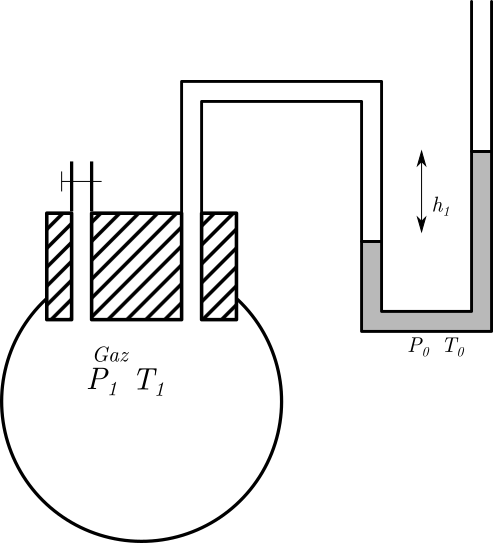
\includegraphics[width=0.8\textwidth]{../fig/calculgamma.png}
	\end{minipage}
	\emph{Indication:} Raisonner sur les n moles restant dans le ballon après la fuite. Lors de la fuite, ces $n$ moles subissent une détente rapide qui pourra être considérée comme adiabatique. De plus comme	$P_1 =  P_0 + \d P$ on pourra la considérer pratiquement quasi-statique et mécaniquement réversible.
\end{Exercise}
\begin{Answer}
	On considère trois état intermédiaires $A,B,C$ avec $0 \to A \xrightarrow{adiabatique} B \xrightarrow{isochore} C $
	Deux méthodes :
	\Question  $PV^\gamma$, puis DL .
	\[\left\{
	\begin{array}{r c l}
		P_AV_A^\gamma&=&P_BV_B^\gamma\\
		P_AV_A&=&P_CV_C
	\end{array}
	\right.
	\Leftrightarrow
	\left\{
	\begin{array}{r c l}
		\left( P_0+h_i \right)V_i^\gamma&=&P_0V_f^\gamma\\
		\left( P_0+h_i \right)V_i&=&\left( P_0+h_f \right)V_f
	\end{array}
	\right.
	\Leftrightarrow
	\left\{
	\begin{array}{r c l}
		\left(\dfrac{V_f}{V_i}\right)^\gamma&=&1+\dfrac{h_i}{P_0}\\
		\dfrac{V_f}{V_i}&=&\dfrac{P_0+h_i}{P_0+h_f}
	\end{array}
	\right.\]
	Et donc,
	\[\Rightarrow 1+\frac{h_i}{P_0}=\left(\frac{P_0+h_i}{P_0+h_f}\right)^\gamma
	=\left(1+\dfrac{h_i}{P_0}\right)^\gamma\left(1+\frac{h_f}{P_0}\right)^{-\gamma}\]
	Comme $\frac{h_i}{P_0} \; \mathrm{et} \; \frac{h_f}{P_0} \ll 1$ :
	\[1+\frac{h_i}{P_0}\approx\left(1+\gamma\dfrac{h_i}{P_0}\right)\left(1-\gamma\dfrac{h_f}{P_0}\right)
	\approx 1+\dfrac{\gamma}{P_0}\left( h_i-h_f \right)\]
	D'où l'expression de $\gamma$ :
	\[\gamma=\frac{h_i}{h_i-h_f}\]
	\Question
	la relation adiabatique donne $P^{1-\gamma}T^\gamma = C^{ste}$ soit en prenant la différentielle logarithmique:
	\[(1-\gamma) \frac{\d P_1}{P} + \gamma \frac{dT}{T} = 0 \]
	Dans la transition isochore on a $PV=nRT $, ie $\frac{P}{T} = C^{ste}$ et de même $\frac{\d P_2 }{P}=\frac{\d T_2}{T}$.

	Or $(\d T = \d T_2)$ donc on a :
	\[(1-\gamma) \frac{\d P_1}{P} =\gamma \frac{\d P_2}{P}\]
	\[\frac{(1-\gamma)}{\gamma} = \dd{P_1}{P_2}  \implies \gamma = \frac{h_1}{h_1-h_2}\]

	Car $h_i = \rho g \d p$
\end{Answer}
